\documentclass{article}

\usepackage[final]{nips_2017}

\usepackage[utf8]{inputenc} % allow utf-8 input
\usepackage[T1]{fontenc}    % use 8-bit T1 fonts
\usepackage{hyperref}       % hyperlinks
\usepackage{url}            % simple URL typesetting
\usepackage{booktabs}       % professional-quality tables
\usepackage{amsfonts}       % blackboard math symbols
\usepackage{nicefrac}       % compact symbols for 1/2, etc.
\usepackage{microtype}      % microtypography
\usepackage{graphicx}
\usepackage{amsmath}
\usepackage{amssymb}

\title{CSE 253 Programming Assignment 1 -- Logistic \& Softmax Regression}

\author{
  Fanjin Zeng \\
  Computer Science and Engineering\\
  University of Califorina, San Diego\\
  \texttt{f1zeng@ucsd.edu} \\
   \And
   Xinyue Ou \\
   Computer Science and Engineering\\
   University of Califorina, San Diego \\
   \texttt{x1ou@ucsd.edu} \\
}

\begin{document}

\maketitle

\section{Derive the gradient for logistic regression}
\begin{equation*}
\begin{gathered}
	E = - \sum_{n=1}^{N}{t^n\ln y^n + (1+t^n) \ln (1-y^n)} \\
	y^n = g_w(x) = \frac{1}{1 + \exp(-w^Tx^n)}\\
	\\
	\frac{\partial E}{\partial y^n} = \frac{1-t^n}{1-y^n}- \frac{t^n}{y^n} = \frac{y^n - t^n}{y^n(1-y^n)}\\
	\frac{\partial y^n}{\partial w} = g_w(x^n) (1-g_w(x^n)) x^n\\
	\\
	\frac{\partial E}{\partial w} = \frac{\partial E}{\partial y^n} \frac{\partial y^n}{\partial w} = (y^n - t^n) x^n	\quad\blacksquare
\end{gathered}
\end{equation*}


\section{Derive the gradient for softmax regression}
\begin{equation*}
\begin{gathered}
	E = - \sum_m \sum_{k=1}^{c} t_k^n \ln y_k^n \\
	y_k^n = \frac{\exp (a_k^n)}{\sum_{k'} \exp(a_{k'}^n)} \\
	a_n^k = w_k^T x^n
\end{gathered}
\end{equation*}

\begin{equation*}
\begin{gathered}
	\frac{\partial y_k^n}{\partial a_k^n} = y_k^n (1 - y_k^n) \\
	\frac{\partial y_k^n}{\partial a_{k''}^n} = - y_k^n y_{k''}^n \quad (k'' \ne k) 
\end{gathered}
\end{equation*}

\begin{equation*}
\begin{split}
	\frac{\partial E}{\partial a_n^k} &= - \sum_{k=1}^{c} t_k^n \frac{1}{y_k^n} \frac{\partial y_k^n}{\partial a_k^n}  \\
	&= -t_k^n + t_k^n y_k^n + \sum_{k' \ne k} y_k^n t_{k'}^n\\
	&= y_k^n \sum_{k'}t_{k'}^n - t_k^n \\
	&= y_k^n - t_k^n
\end{split}
\end{equation*}

\begin{equation*}
	\dfrac{\mathrm{d} a_k^n}{\mathrm{d} w_{jk}} = x_j^n
\end{equation*}

\begin{equation*}
\begin{split}
	\frac{\partial E}{\partial w_{jk}} &= \frac{\partial E}{\partial a_n^k} \frac{\partial a_k^n}{\partial w_{jk}} \\
	&= (y_k^n - t_k^n) x_j^n \quad\blacksquare
\end{split}
\end{equation*}

\section{Read in data}
After getting the dataset from \href{http://yann.lecun.com/exdb/mnist/}{this page}, we read it into our program by unpacking it to desired structure. According to the file format description, for image data, the first 16 bytes are the magic number, the size, the row and the column, followed by the actual data. For the label data, the first 8 bytes are the magic number and the size.

For convenience, we reshape the train and test image data into 784 * (Number of images). In softmax regression, we encode train and test labels using one-hot scheme. In logistic regression, we relabeled train and test labels as True or False, based on whether they belong to desired category.

We use the first 20,000 training images and the first 2,000 testing images.

\section{Logistic regression via gradient descent}
\subsection{Problem abstract}
In this section, our object is to use logistic regression to classify 2 categories of handwritten digits. We use gradient descent technique to train the weight, and mini-batch to get faster convergence. We also experiment annealing, early stop, and regularization to achieve better generalization.

\subsection{Further discussion}
\subsubsection{}
\subsubsection{}
\subsubsection{Repeat exercise for 2 vs. 8}
\subsubsection{Display weights images}

\subsubsection{Implementation}
\subsubsection{Result}
\subsection{Epilogue}

\section{Regulation}
\subsection{Problem abstract}
Sometimes the regression model suffers from over fit, which reduces the generalization of the model. This can be improved by introducing regularization part to the loss function. With the cost function becoming \begin{align*}
J(w) = E(w) + \lambda C(w)
\end{align*}
 the loss function is penalized by the complexity of model parametrized by value $\lambda$. There are two major forms of regularization. 
 
 $L_1:$\begin{align*}
  C(w) = ||w||
  \end{align*}
 $L_2:$\begin{align*}
 C(w) = ||w||^2
 \end{align*}
\subsection{Discussion}
\subsubsection*{(a)} 
To derive the gradient descent of the two types of regularizations, we have 

$L_1$: \begin{align*}
\frac{d}{dw_j}C(w) = sgn(w_j) 
\end{align*}
$L_2$: \begin{align*}
\frac{d}{dw_j}C(w) = 2w_j 
\end{align*}
\subsubsection*{(b)} 
To figure out the best $\lambda$ to regularize the weight, we train our model against the lambda value of 0.0001, 0.001, 0.01, 0.1 and 1, and two types of regularization respectively.
\begin{figure}[h]
	\centering
	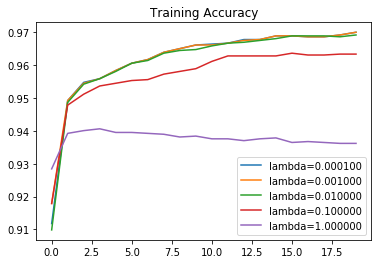
\includegraphics[scale = 0.7]{pics/lambda_train_1.png}
	\caption{L1 regularization. Model accuracy vs training epochs, with different values of lambda}
\end{figure}
\begin{figure}[h]
	\centering
	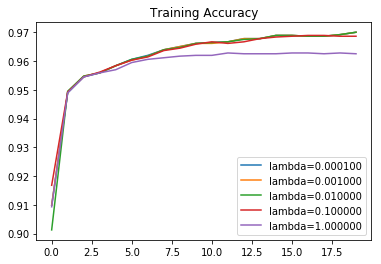
\includegraphics[scale = 0.7]{pics/lambda_train_2.png}
	\caption{L2 regularization. Model accuracy vs training epochs, with different values of lambda}
\end{figure}

From the figures we can observe, as lambda increases, the accuracy of training set decreases. It actually coincides with the intention to use regularization to penalize the overfitting of training set. As more regularization put on the training set, the model will not train into a state that over compliments the training data. Therefore it should not fit the training data that much when lambda goes up.

We also observe that the L1 regularization poses more penalty than the L2. It may be due to the fact that the absolute value of most of the weights here are far less than 1, making L1 regularization has a more significant effect than L2.
\subsubsection*{(c)}
To see the actual effect that regularization poses on weight, we plot the 2-norm of the weight versus the values of lambda. As observed, the weight keeps going down as the lambda goes up. It makes sense since the increase of lambda poses more penalty on the weight to keep the model free from large weights. 

\begin{figure}[h]
	\begin{minipage}{0.48\textwidth}
		\centering
		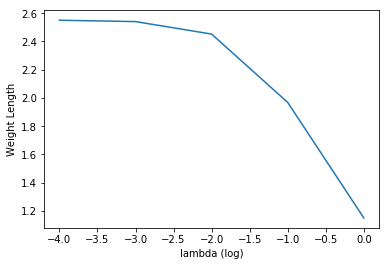
\includegraphics[width=\textwidth]{pics/weight_1.png}
		\caption{L1 regularization. Weight vector vs lambda}
	\end{minipage}\hfill
	\begin {minipage}{0.48\textwidth}
	\centering
		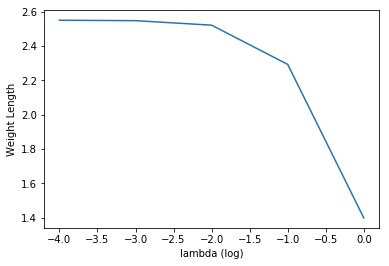
\includegraphics[width=\textwidth]{pics/weight_2.png}
		\caption{L2 regularization.  Weight vector vs lambda}
\end{minipage}
\end{figure}
\subsubsection*{(d)}
We then want to check the practical values of using regularization. By testing the regularized model on the testing data, we obtain the error rate of the model respectively for L1 and L2 regularization.
\begin{figure}[h]
	\begin{minipage}{0.48\textwidth}
		\centering
	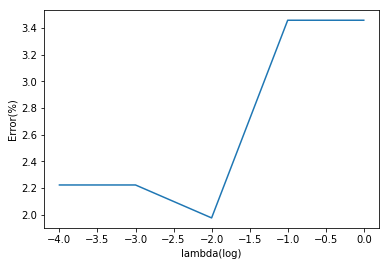
\includegraphics[width=\textwidth]{pics/lambda_test_1.png}
	\caption{L1 regularization. Test error versus lambda}
	\end{minipage}\hfill
	\begin {minipage}{0.48\textwidth}
	\centering
	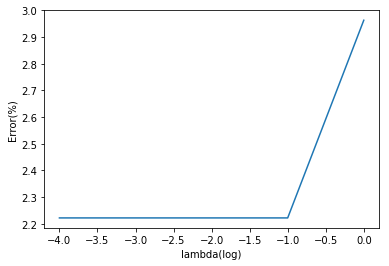
\includegraphics[width=\textwidth]{pics/lambda_test_2.png}
	\caption{L2 regularization. Test error versus lambda}
\end{minipage}
\end{figure}


As we can observed, the best lambda for L1 regularization is when $\lambda = 10^{-2}$, and $\lambda < 10^{-1}$ for L2. It makes sense that the regularization first helps with the generalization of the model that it prevents overfitting on the training data. Hence the error on the test set goes down when lambda goes up. Nonetheless, the increasing of lambda also impedes the pace of gradient descent that makes the model become under-trained. Hence we can observe an increase in error when lambda keeps going up.

The best lambda for our model is $\lambda=10^{-2}$ 
\subsubsection*{(e)}
\begin{figure}[h]
	\centering
	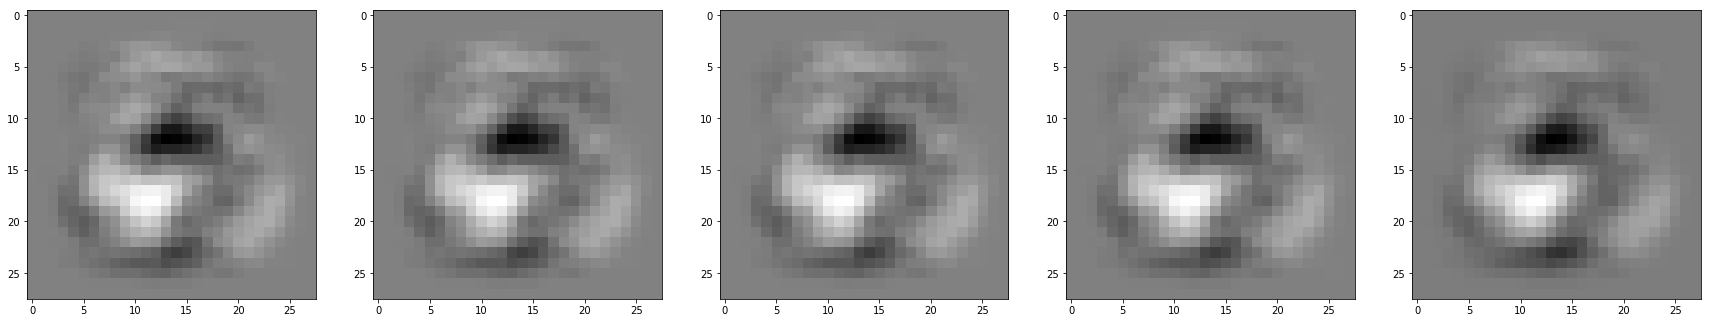
\includegraphics[width=\textwidth]{pics/weight_img.png}
	\caption{Weight images with different lambda. Lambda increases from left to right}
\end{figure}
Through the weight images, we can observe that with higher lambda, the weight image is actually more blurred than the one with lower lambda. There are mode granule details in images with lower lambda. This is may because the weights in lower lambda image can grow more freely than the one with higher lambda.
\section{Softmax regression via gradient descent}
\subsection{Problem abstract}
The following section will focus on using the technique we have mention above to apply to all categories of hand-written digits. Softmax is the activation function we use in this application. It is an extension of the sigmoid function we used in Logistic Regression. Note that the softmax function is \begin{align*}
y_k^n =\frac{exp(a_k^n)}{\sum_{k'} exp(a_k'^n )}
\end{align*}

\subsection{Discussion}
\subsubsection*{(a)}
We first find the best lambda and regularization for the softmax model. 
\begin{figure}[h]
	\begin{minipage}{0.48\textwidth}
		\centering
		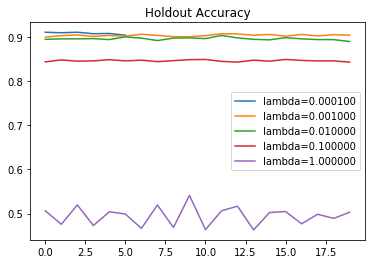
\includegraphics[width=\textwidth]{pics/softmax_reg_1.png}
		\caption{L1 regularization. Holdout  accuracy over training. Early stop enabled.}
	\end{minipage}\hfill
	\begin {minipage}{0.48\textwidth}
	\centering
	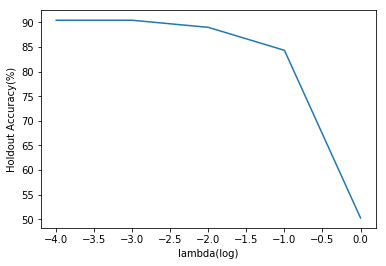
\includegraphics[width=\textwidth]{pics/softmax_reg_2.png}
	\caption{L1 regularization. Holdout accuracy vs lambda. Early stop enabled.}
\end{minipage}
\end{figure}
For L1 regularization, the holdout set has a highest accuracy when $\lambda=0.001$.
\begin{figure}[h]
	\begin{minipage}{0.48\textwidth}
		\centering
		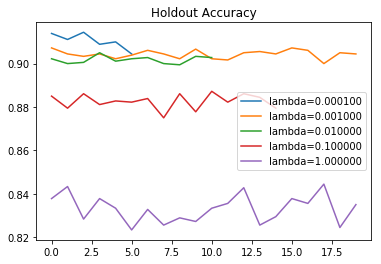
\includegraphics[width=\textwidth]{pics/softmax_reg_3.png}
		\caption{L2 regularization. Holdout  accuracy over training. Early stop enabled.}
	\end{minipage}\hfill
	\begin {minipage}{0.48\textwidth}
	\centering
	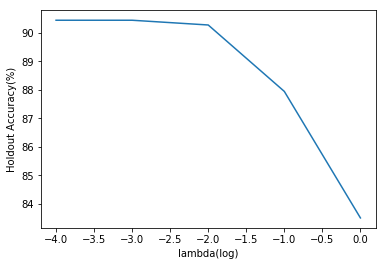
\includegraphics[width=\textwidth]{pics/softmax_reg_4.png}
	\caption{L2 regularization. Holdout accuracy vs lambda. Early stop enabled.}
\end{minipage}
\end{figure}
For L2 regularization, the holdout set has a highest accuracy when $\lambda=0.001$.

Note that the two kinds of regularization does not has a significant difference when $\lambda$ is low. However, as $\lambda$ increases in magnitude, the L1 regularization significantly impedes the accuracy, given its larger value compared to L2. We choose L2 for stabler result in general cases.
For the best case

\subsubsection{(b)}
Training accuracy 92.688889 %, Val accuracy 92.650000 %, Test accuracy: 93.600000 %
With L2 regularization and $\lambda=0.001$, we train the model to classify 10 hand written digits. The training loss is 0.4191, the holdout loss is 0.2726and the test loss is 0.2078.
\begin{figure}[h]
	\centering
	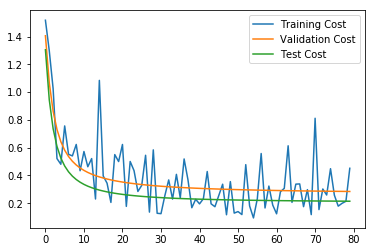
\includegraphics[width=0.7\textwidth]{pics/softmax_best_loss.png}
	\caption{The loss function plot versus every 20 training epochs for the trained softmax model. $\lambda =0.001$, L2 regularization, learning rate = 0.001. }
\end{figure}

\subsubsection{(c)}
With L2 regularization and $\lambda=0.001$, we train the model to classify 10 hand written digits. Training accuracy 92.688889 \%, val accuracy 92.650000 \%, and test accuracy: 93.600000 \%
\begin{figure}[h]
	\centering
	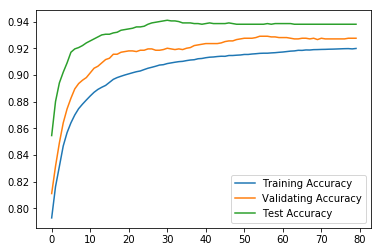
\includegraphics[width=0.7\textwidth]{pics/softmax_best_accuracy.png}
	\caption{The accuracy plot versus every 20 training epochs for the trained softmax model. $\lambda =0.001$, L2 regularization, learning rate = 0.001. }
\end{figure}

\subsubsection{(d)}

We plot the weight for each category and its corresponding average image in the training set.

\begin{figure}[thbp]
	\begin{minipage}{0.48\textwidth}
		\centering
		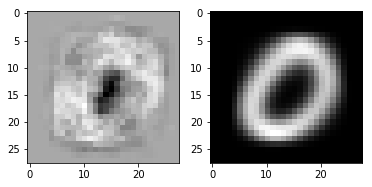
\includegraphics[width=\textwidth]{pics/0.png}
		\caption{Weight for category 0 and the average weight of 0 in training set}
	\end{minipage}\hfill
	\begin {minipage}{0.48\textwidth}
	\centering
	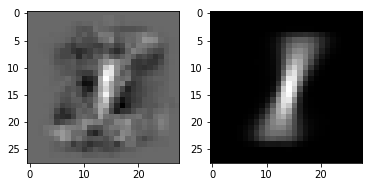
\includegraphics[width=\textwidth]{pics/1.png}
	\caption{Weight for category 1 and the average weight of 1 in training set}
\end{minipage}
	\begin{minipage}{0.48\textwidth}
		\centering
		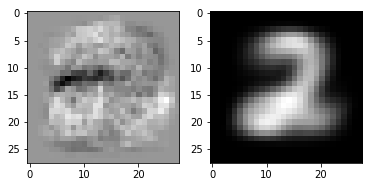
\includegraphics[width=\textwidth]{pics/2.png}
		\caption{Weight for category 2 and the average weight of 2 in training set}
	\end{minipage}\hfill
	\begin {minipage}{0.48\textwidth}
	\centering
	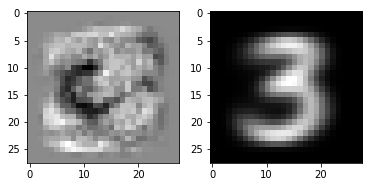
\includegraphics[width=\textwidth]{pics/3.png}
	\caption{Weight for category 3 and the average weight of 3 in training set}
\end{minipage}
	\begin{minipage}{0.48\textwidth}
		\centering
		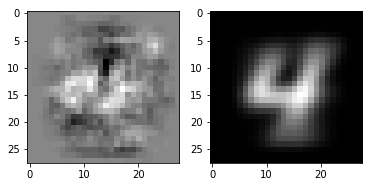
\includegraphics[width=\textwidth]{pics/4.png}
		\caption{Weight for category 4 and the average weight of 4 in training set}
	\end{minipage}\hfill
	\begin {minipage}{0.48\textwidth}
	\centering
	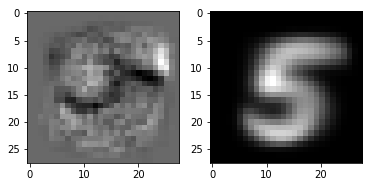
\includegraphics[width=\textwidth]{pics/5.png}
	\caption{Weight for category 5 and the average weight of 5 in training set}
\end{minipage}
	\begin{minipage}{0.48\textwidth}
		\centering
		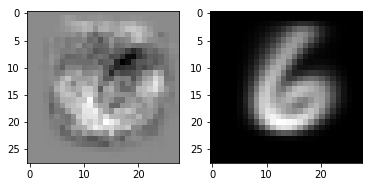
\includegraphics[width=\textwidth]{pics/6.png}
		\caption{Weight for category 6 and the average weight of 6 in training set}
	\end{minipage}\hfill
	\begin {minipage}{0.48\textwidth}
	\centering
	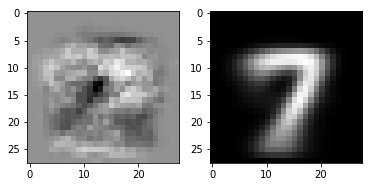
\includegraphics[width=\textwidth]{pics/7.png}
	\caption{Weight for category 7 and the average weight of 7 in training set}
\end{minipage}
	\begin{minipage}{0.48\textwidth}
		\centering
		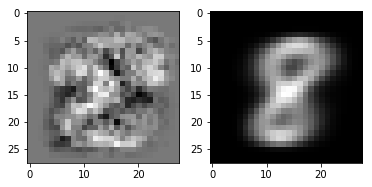
\includegraphics[width=\textwidth]{pics/8.png}
		\caption{Weight for category 8 and the average weight of 8 in training set}
	\end{minipage}\hfill
	\begin {minipage}{0.48\textwidth}
	\centering
	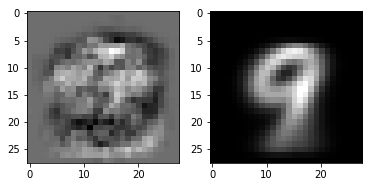
\includegraphics[width=\textwidth]{pics/9.png}
	\caption{Weight for category 9 and the average weight of 9 in training set}
\end{minipage}
\end{figure}


\section{Summary}
To conclude, in this assignment, we first use logistic regression to discriminate digits of two categories. After experiment, we settle on the learning rate of 0.001 and the L2 regularization with parameter $\lambda = 0.001$ for our training task. We achieve a best result of 98.02\% accuracy on digits 2 and 3 and 96.10\% on 2 and 8. For the softmax task, we use a learning rate of 0.00001 and L2 regularization with  $\lambda = 0.001$, and achieve a accuracy of 93.60 \% on all ten categories.

From this assignment, we learn how to implement logistic and softmax regression. Through comparison and experimenting, we discover the effects of different parameters and the rationale behind each effect. 
\section{Contributions}


Xinyue Ou is in charged of the regularization experimenting and softmax regression. He wrote part of the codes to help better illustrate the results we obtain in the model.
\section{References}
[1] Bishop, C. M., {\it Neural networks for pattern recognition}, Oxford: Oxford University Press, 2013.
\end{document}










% The following part is displayed



\section{Submission of papers to NIPS 2017}

NIPS requires electronic submissions.  The electronic submission site
is
\begin{center}
  \url{https://cmt.research.microsoft.com/NIPS2017/}
\end{center}

Please read carefully the instructions below and follow them
faithfully.

\subsection{Style}

Papers to be submitted to NIPS 2017 must be prepared according to the
instructions presented here. Papers may only be up to eight pages
long, including figures. This does not include acknowledgments and 
cited references which are allowed on subsequent pages.

The margins in 2017 are the same as since 2007, which allow for
$\sim$$15\%$ more words in the paper compared to earlier years.

Authors are required to use the NIPS \LaTeX{} style files obtainable
at the NIPS website as indicated below. 

\subsection{Retrieval of style files}

The style files for NIPS and other conference information are
available on the World Wide Web at
\begin{center}
  \url{http://www.nips.cc/}
\end{center}
The file \verb+nips_2017.pdf+ contains these instructions and
illustrates the various formatting requirements your NIPS paper must
satisfy.

The only supported style file for NIPS 2017 is \verb+nips_2017.sty+,
rewritten for \LaTeXe{}.  \textbf{Previous style files for \LaTeX{}
  2.09, Microsoft Word, and RTF are no longer supported!}

The new \LaTeX{} style file contains two optional arguments:
\verb+final+, which creates a camera-ready copy, and \verb+nonatbib+,
which will not load the \verb+natbib+ package for you in case of
package clash.

At submission time, please omit the \verb+final+ option. This will
anonymize your submission and add line numbers to aid review.  Please
do \emph{not} refer to these line numbers in your paper as they will
be removed during generation of camera-ready copies.

The file \verb+nips_2017.tex+ may be used as a ``shell'' for writing
your paper. All you have to do is replace the author, title, abstract,
and text of the paper with your own.

The formatting instructions contained in these style files are
summarized in Sections \ref{gen_inst}, \ref{headings}, and
\ref{others} below.

\section{General formatting instructions}
\label{gen_inst}

The text must be confined within a rectangle 5.5~inches (33~picas)
wide and 9~inches (54~picas) long. The left margin is 1.5~inch
(9~picas).  Use 10~point type with a vertical spacing (leading) of
11~points.  Times New Roman is the preferred typeface throughout, and
will be selected for you by default.  Paragraphs are separated by
\nicefrac{1}{2}~line space (5.5 points), with no indentation.

The paper title should be 17~point, initial caps/lower case, bold,
centered between two horizontal rules. The top rule should be 4~points
thick and the bottom rule should be 1~point thick. Allow
\nicefrac{1}{4}~inch space above and below the title to rules. All
pages should start at 1~inch (6~picas) from the top of the page.

For the final version, authors' names are set in boldface, and each
name is centered above the corresponding address. The lead author's
name is to be listed first (left-most), and the co-authors' names (if
different address) are set to follow. If there is only one co-author,
list both author and co-author side by side.

Please pay special attention to the instructions in Section \ref{others}
regarding figures, tables, acknowledgments, and references.

\section{Headings: first level}
\label{headings}

All headings should be lower case (except for first word and proper
nouns), flush left, and bold.

First-level headings should be in 12-point type.

\subsection{Headings: second level}

Second-level headings should be in 10-point type.

\subsubsection{Headings: third level}

Third-level headings should be in 10-point type.

\paragraph{Paragraphs}

There is also a \verb+\paragraph+ command available, which sets the
heading in bold, flush left, and inline with the text, with the
heading followed by 1\,em of space.

\section{Citations, figures, tables, references}
\label{others}

These instructions apply to everyone.

\subsection{Citations within the text}

The \verb+natbib+ package will be loaded for you by default.
Citations may be author/year or numeric, as long as you maintain
internal consistency.  As to the format of the references themselves,
any style is acceptable as long as it is used consistently.

The documentation for \verb+natbib+ may be found at
\begin{center}
  \url{http://mirrors.ctan.org/macros/latex/contrib/natbib/natnotes.pdf}
\end{center}
Of note is the command \verb+\citet+, which produces citations
appropriate for use in inline text.  For example,
\begin{verbatim}
   \citet{hasselmo} investigated\dots
\end{verbatim}
produces
\begin{quote}
  Hasselmo, et al.\ (1995) investigated\dots
\end{quote}

If you wish to load the \verb+natbib+ package with options, you may
add the following before loading the \verb+nips_2017+ package:
\begin{verbatim}
   \PassOptionsToPackage{options}{natbib}
\end{verbatim}

If \verb+natbib+ clashes with another package you load, you can add
the optional argument \verb+nonatbib+ when loading the style file:
\begin{verbatim}
   \usepackage[nonatbib]{nips_2017}
\end{verbatim}

As submission is double blind, refer to your own published work in the
third person. That is, use ``In the previous work of Jones et
al.\ [4],'' not ``In our previous work [4].'' If you cite your other
papers that are not widely available (e.g., a journal paper under
review), use anonymous author names in the citation, e.g., an author
of the form ``A.\ Anonymous.''

\subsection{Footnotes}

Footnotes should be used sparingly.  If you do require a footnote,
indicate footnotes with a number\footnote{Sample of the first
  footnote.} in the text. Place the footnotes at the bottom of the
page on which they appear.  Precede the footnote with a horizontal
rule of 2~inches (12~picas).

Note that footnotes are properly typeset \emph{after} punctuation
marks.\footnote{As in this example.}

\subsection{Figures}

All artwork must be neat, clean, and legible. Lines should be dark
enough for purposes of reproduction. The figure number and caption
always appear after the figure. Place one line space before the figure
caption and one line space after the figure. The figure caption should
be lower case (except for first word and proper nouns); figures are
numbered consecutively.

You may use color figures.  However, it is best for the figure
captions and the paper body to be legible if the paper is printed in
either black/white or in color.
\begin{figure}[h]
  \centering
  \fbox{\rule[-.5cm]{0cm}{4cm} \rule[-.5cm]{4cm}{0cm}}
  \caption{Sample figure caption.}
\end{figure}

\subsection{Tables}

All tables must be centered, neat, clean and legible.  The table
number and title always appear before the table.  See
Table~\ref{sample-table}.

Place one line space before the table title, one line space after the
table title, and one line space after the table. The table title must
be lower case (except for first word and proper nouns); tables are
numbered consecutively.

Note that publication-quality tables \emph{do not contain vertical
  rules.} We strongly suggest the use of the \verb+booktabs+ package,
which allows for typesetting high-quality, professional tables:
\begin{center}
  \url{https://www.ctan.org/pkg/booktabs}
\end{center}
This package was used to typeset Table~\ref{sample-table}.

\begin{table}[t]
  \caption{Sample table title}
  \label{sample-table}
  \centering
  \begin{tabular}{lll}
    \toprule
    \multicolumn{2}{c}{Part}                   \\
    \cmidrule{1-2}
    Name     & Description     & Size ($\mu$m) \\
    \midrule
    Dendrite & Input terminal  & $\sim$100     \\
    Axon     & Output terminal & $\sim$10      \\
    Soma     & Cell body       & up to $10^6$  \\
    \bottomrule
  \end{tabular}
\end{table}

\section{Final instructions}

Do not change any aspects of the formatting parameters in the style
files.  In particular, do not modify the width or length of the
rectangle the text should fit into, and do not change font sizes
(except perhaps in the \textbf{References} section; see below). Please
note that pages should be numbered.

\section{Preparing PDF files}

Please prepare submission files with paper size ``US Letter,'' and
not, for example, ``A4.''

Fonts were the main cause of problems in the past years. Your PDF file
must only contain Type 1 or Embedded TrueType fonts. Here are a few
instructions to achieve this.

\begin{itemize}

\item You should directly generate PDF files using \verb+pdflatex+.

\item You can check which fonts a PDF files uses.  In Acrobat Reader,
  select the menu Files$>$Document Properties$>$Fonts and select Show
  All Fonts. You can also use the program \verb+pdffonts+ which comes
  with \verb+xpdf+ and is available out-of-the-box on most Linux
  machines.

\item The IEEE has recommendations for generating PDF files whose
  fonts are also acceptable for NIPS. Please see
  \url{http://www.emfield.org/icuwb2010/downloads/IEEE-PDF-SpecV32.pdf}

\item \verb+xfig+ "patterned" shapes are implemented with bitmap
  fonts.  Use "solid" shapes instead.

\item The \verb+\bbold+ package almost always uses bitmap fonts.  You
  should use the equivalent AMS Fonts:
\begin{verbatim}
   \usepackage{amsfonts}
\end{verbatim}
followed by, e.g., \verb+\mathbb{R}+, \verb+\mathbb{N}+, or
\verb+\mathbb{C}+ for $\mathbb{R}$, $\mathbb{N}$ or $\mathbb{C}$.  You
can also use the following workaround for reals, natural and complex:
\begin{verbatim}
   \newcommand{\RR}{I\!\!R} %real numbers
   \newcommand{\Nat}{I\!\!N} %natural numbers
   \newcommand{\CC}{I\!\!\!\!C} %complex numbers
\end{verbatim}
Note that \verb+amsfonts+ is automatically loaded by the
\verb+amssymb+ package.

\end{itemize}

If your file contains type 3 fonts or non embedded TrueType fonts, we
will ask you to fix it.

\subsection{Margins in \LaTeX{}}

Most of the margin problems come from figures positioned by hand using
\verb+\special+ or other commands. We suggest using the command
\verb+\includegraphics+ from the \verb+graphicx+ package. Always
specify the figure width as a multiple of the line width as in the
example below:
\begin{verbatim}
   \usepackage[pdftex]{graphicx} ...
   \includegraphics[width=0.8\linewidth]{myfile.pdf}
\end{verbatim}
See Section 4.4 in the graphics bundle documentation
(\url{http://mirrors.ctan.org/macros/latex/required/graphics/grfguide.pdf})

A number of width problems arise when \LaTeX{} cannot properly
hyphenate a line. Please give LaTeX hyphenation hints using the
\verb+\-+ command when necessary.

\subsubsection*{Acknowledgments}

Use unnumbered third level headings for the acknowledgments. All
acknowledgments go at the end of the paper. Do not include
acknowledgments in the anonymized submission, only in the final paper.

\section*{References}

References follow the acknowledgments. Use unnumbered first-level
heading for the references. Any choice of citation style is acceptable
as long as you are consistent. It is permissible to reduce the font
size to \verb+small+ (9 point) when listing the references. {\bf
  Remember that you can go over 8 pages as long as the subsequent ones contain
  \emph{only} cited references.}
\medskip

\small

[1] Alexander, J.A.\ \& Mozer, M.C.\ (1995) Template-based algorithms
for connectionist rule extraction. In G.\ Tesauro, D.S.\ Touretzky and
T.K.\ Leen (eds.), {\it Advances in Neural Information Processing
  Systems 7}, pp.\ 609--616. Cambridge, MA: MIT Press.

[2] Bower, J.M.\ \& Beeman, D.\ (1995) {\it The Book of GENESIS:
  Exploring Realistic Neural Models with the GEneral NEural SImulation
  System.}  New York: TELOS/Springer--Verlag.

[3] Hasselmo, M.E., Schnell, E.\ \& Barkai, E.\ (1995) Dynamics of
learning and recall at excitatory recurrent synapses and cholinergic
modulation in rat hippocampal region CA3. {\it Journal of
  Neuroscience} {\bf 15}(7):5249-5262.

